\documentclass[leqno]{article}
% Shared QBT/Soln pack preamble for resources.danieljsmith.org.
\usepackage{graphicx}
\usepackage{dsfont}
\usepackage{mathtools}
\usepackage{amssymb}
\usepackage{amsmath}
\usepackage{mleftright}
\usepackage{amsthm}
\usepackage{float}
\usepackage{ragged2e}
\usepackage{tensor}
\usepackage{fancyhdr}
\usepackage{empheq}
\usepackage[most]{tcolorbox}
\usepackage{enumitem}
\usepackage{dirtytalk}
\usepackage{marginnote}
\usepackage{microtype}
\usepackage[
  a4paper,
  left=0.8in,
  right=1in,
  top=1in,
  bottom=0.5in,
  headheight=14pt,
  headsep=0.4in
]{geometry}
\setlength{\parindent}{0cm}

% TikZ / PGFPlots
\usepackage{pgfplots}
\pgfplotsset{compat=1.18}
\usepgfplotslibrary{fillbetween, polar}
\usetikzlibrary{calc, positioning}
\usetikzlibrary{angles, quotes}
\usetikzlibrary{arrows.meta}
\usetikzlibrary{decorations.pathreplacing, decorations.markings}
\usetikzlibrary{patterns}
\usetikzlibrary{intersections}

% Links and contents. The contents follow the TMUA papers: compact entries,
% no dot leaders, and each question's mark total in grey after its label.
\usepackage{tocloft}
\tocloftpagestyle{fancy}
\setlength{\cftbeforesubsecskip}{2pt}
\setlength{\cftsubsecindent}{1.5em}
\setlength{\cftsubsecnumwidth}{0pt}
\renewcommand{\cftsubsecfont}{\small\color{black}}
\renewcommand{\cftsubsecpagefont}{\small\color{black}}
\renewcommand{\cftsubsecleader}{\hfill}
\usepackage[colorlinks=true,linkcolor=black,citecolor=magenta,urlcolor=black]{hyperref}%
\urlstyle{same}

% Pack macros
% \marks also adds its value to the current question's total in the .aux
% file, so the contents show each total from the second pass. The write
% happens at shipout, so a box typeset more than once counts once. The
% pack's mark total for the contents-page title is summed the same way.
\makeatletter
\newcount\djs@totalmarks
\newcommand{\djsAddMarks}[2]{%
  \global\advance\djs@totalmarks#2\relax
  \@ifundefined{djs@marks@#1}%
    {\expandafter\xdef\csname djs@marks@#1\endcsname{#2}}%
    {\expandafter\xdef\csname djs@marks@#1\endcsname
      {\the\numexpr\csname djs@marks@#1\endcsname+#2\relax}}}
\RenewDocumentCommand{\marks}{o m}{%
  \protected@write\@auxout{}{\string\djsAddMarks{\number\value{enumi}}{#2}}%
  \IfValueTF{#1}%
    {\marginnote{\raggedright\textbf{[#2]}}[#1]}%
    {\marginnote{\raggedright\textbf{[#2]}}}%
}
\makeatother

\newcommand{\vspacerule}[2]{%
  \par\vspace*{#1}%
  \noindent\hrulefill\par
  \vspace*{#2}%
}

\definecolor{scarlet}{RGB}{205, 40, 75}
% Site colours for the contents-page title: the accent, the rule colour, a
% stronger rule colour for the path separator, and the muted text colour.
\definecolor{djsBurgundy}{RGB}{118, 59, 67}
\definecolor{djsHairline}{RGB}{216, 213, 205}
\definecolor{djsSlash}{RGB}{170, 166, 158}
\definecolor{djsMuted}{RGB}{96, 101, 106}

% Worked-solution box, adapted from the TMUA worked-solutions box. A white breakable box with a left scarlet rule and no surrounding
% frame or tint. A part that breaks fills the rest of its page, so the rule
% runs to the bottom margin; the unbroken or last part ends in a short
% horizontal foot rule so a solution visibly stops. Unlike the TMUA box there
% is no answer label. The box does not grow to the left, so the rule sits at
% the text edge; growing to the right keeps the usable line width close to the
% old tcolorbox Solution box.
% Spacing inside the box: paragraphs are 6pt apart, so source blank lines show
% (solutions put one after each display and none between a lead-in and its
% display). Every display gets 6pt above and 10pt below, whatever the length
% of its lead-in line; align rows are spread by an 8pt \jot; solution parts
% are 14pt apart and sub-parts 8pt; \left and \right space like ordinary
% brackets (mleftright); no single line is stranded at a page break; and
% neither the Solution label nor the line before a list ends a page. No
% skip can shrink, so full pages are not squeezed.
\newtcolorbox{djsSolution}{%
  enhanced, breakable, frame hidden, sharp corners, colback=white,
  height fixed for=first and middle, height fill,
  extras unbroken and last={natural height},
  borderline west={2.2pt}{0pt}{scarlet},
  left=11pt, right=0pt, top=5pt, bottom=13pt,
  before skip=13pt, after skip=4pt,
  grow to right by=10mm,
  overlay unbroken and last={%
    \fill[scarlet] (frame.south west)
      rectangle ([xshift=3.5cm, yshift=2.2pt]frame.south west);},
  before upper={{\color{scarlet}\bfseries Solution}\par\nobreak\vspace{4pt}%
    \setlength{\parskip}{6pt plus 2pt}%
    \setlength{\abovedisplayskip}{6pt plus 2pt}%
    \setlength{\abovedisplayshortskip}{6pt plus 2pt}%
    \setlength{\belowdisplayskip}{10pt plus 2pt}%
    \setlength{\belowdisplayshortskip}{10pt plus 2pt}%
    \setlength{\jot}{8pt}%
    \setlist{parsep=6pt plus 2pt, topsep=6pt plus 2pt, beginpenalty=10000}%
    \setlist[enumerate,1]{itemsep=14pt plus 2pt}%
    \setlist[enumerate,2]{itemsep=8pt plus 2pt}%
    \mleftright
    \clubpenalty=10000 \widowpenalty=10000 \displaywidowpenalty=10000\relax}}

% Optional smaller figure inside a solution box. \scalebox shrinks node text
% with the drawing. Not applied to existing figures.
\newcommand{\SolnFigureScale}{0.85}
\newsavebox{\djsSolnFigureBox}
\newenvironment{djsSolutionFigure}
  {\par\vspace{4pt}\begin{center}\begin{lrbox}{\djsSolnFigureBox}}
  {\end{lrbox}\scalebox{\SolnFigureScale}{\usebox{\djsSolnFigureBox}}%
   \end{center}\vspace{2pt}\par}

\newcommand{\cxl}[2]{%
  \tikz[baseline=(X.base)]{%
    \node[inner sep=0pt, outer sep=0pt, text=#1] (X) {$#2$};
    \draw[#1, line width=0.4pt] (X.south west)--(X.north east);
  }%
}

% Page-style hook run at the contents page and each question's opening page.
% A no-op for QBT packs; \djsSolnHeader points it at the fancy header.
\newcommand{\djsQuestionPageStyle}{}

% A contents entry: "Question N" in a box wide enough for two digits, so the
% mark totals line up, then the total in grey. Bookmarks keep "Question N".
\makeatletter
\newlength{\djsTocLabelWidth}
\newcommand{\djsTocMarks}[1]{%
  \@ifundefined{djs@marks@#1}{}{%
    {\footnotesize\itshape\color{black!45}%
     \csname djs@marks@#1\endcsname~mark%
     \ifnum\csname djs@marks@#1\endcsname=1 \else s\fi}}}
\newcommand{\djsTocEntry}[1]{%
  \texorpdfstring
    {\settowidth{\djsTocLabelWidth}{Question 00}%
     \makebox[\dimexpr\djsTocLabelWidth+0.9em\relax][l]{Question #1}%
     \djsTocMarks{#1}}%
    {Question #1}}
\makeatother

% The question count for the contents-page title is written to the .aux at
% the end of the document, so it also appears from the second pass.
\newcounter{djsQuestions}
\newcommand{\questionitem}{%
  \djsQuestionPageStyle
  \item\phantomsection
  \stepcounter{djsQuestions}%
  \addcontentsline{toc}{subsection}{\protect\djsTocEntry{\number\value{enumi}}}%
}
\makeatletter
\newcommand{\djsSetQuestionCount}[1]{\gdef\djs@questioncount{#1}}
\AtEndDocument{\immediate\write\@auxout
  {\string\djsSetQuestionCount{\number\value{djsQuestions}}}}
\makeatother

\renewcommand{\contentsname}{Questions}

% \djsPackHeader[<link content tag>]{<left header>}; the tag says which
% document a click on the header link came from.
\newcommand{\djsPackHeader}[2][questions]{%
  \pagestyle{fancy}%
  \fancyhead{}%
  \fancyfoot{}%
  \renewcommand{\headrulewidth}{0.9pt}%
  \lhead{#2}%
  \chead{}%
  \rhead{\href{https://danieljsmith.org/?utm_source=pdf&utm_campaign=further-maths&utm_content=#1}{danieljsmith.org}}%
}

% The header's topic is also the contents-page title, under which a label
% says which booklet this is.
\newcommand{\djsPackTitle}{}
\newcommand{\djsBookletLabel}{}
\newcommand{\djsQbtHeader}[1]{%
  \djsPackHeader{#1}%
  \renewcommand{\djsPackTitle}{#1}%
  \renewcommand{\djsBookletLabel}{Questions by topic}%
}

% The colophon at the foot of page one, independent of the page style: the
% contents-page title's hairline led by a short scarlet rule, then the date on
% the left and a link to the site on the right, all inside the bottom margin.
% Its sizes are fixed, so it matches the TMUA papers' colophon. The document
% supplies the date; recompiling never changes it.
\makeatletter
\newcommand{\djsLastUpdated}[1]{%
  \AtBeginDocument{\AddToHookNext{shipout/foreground}{\djs@colophon{#1}}}}
\newcommand{\djs@colophon}[1]{%
  \put(0.8in,-\dimexpr\paperheight-0.47in\relax){%
    \makebox[0pt][l]{\color{djsHairline}%
      \rule[0.9pt]{\dimexpr\paperwidth-1.8in\relax}{0.6pt}}%
    \makebox[0pt][l]{\color{scarlet}\rule{3.5cm}{2.2pt}}}%
  \put(0.8in,-\dimexpr\paperheight-0.32in\relax){\makebox[0pt][l]{%
    \fontsize{9}{11}\selectfont Last updated #1}}%
  \put(\dimexpr\paperwidth-1in\relax,-\dimexpr\paperheight-0.32in\relax){%
    \makebox[0pt][r]{\fontsize{7}{8.5}\selectfont\color{djsMuted}%
      Latest version at \href{https://resources.danieljsmith.org/}%
        {\color{black}resources.danieljsmith.org}}}}
\makeatother

% Solutions packs show the header only on the contents page and each
% question's opening page, so it never appears part-way through a solution.
% \thispagestyle marks the next page shipped out, which is the question's
% page because every solution question starts after a \newpage.
\newcommand{\djsSolnHeader}[1]{%
  \djsPackHeader[solutions]{\textit{Solutions} - #1}%
  \pagestyle{empty}%
  \renewcommand{\djsQuestionPageStyle}{\thispagestyle{fancy}}%
  \renewcommand{\djsPackTitle}{#1}%
  \renewcommand{\djsBookletLabel}{Worked solutions}%
}

% \djsSitePath{<strand>}{<topic>}, called once after the header, names where
% the pack sits on the site; the contents-page title prints it above the pack
% title, e.g. CORE PURE / FURTHER CALCULUS. Without it the line is left out.
\makeatletter
\newif\ifdjs@sitepath
\newcommand{\djs@strand}{}
\newcommand{\djs@section}{}
\newcommand{\djsSitePath}[2]{%
  \djs@sitepathtrue
  \renewcommand{\djs@strand}{#1}%
  \renewcommand{\djs@section}{#2}%
}
\makeatother

% Further Mechanics packs call \djsMechanicsPack in their preamble, so that
% \djsFrontMatter prints the default value of g above the contents. The box
% keeps its own space above it (before skip is the whole gap below the title,
% not an addition to it). Without the box, \djsGravityNote is just extra space
% before the contents heading, bringing the gap above it close to the gap
% between the box and the heading on Further Mechanics pages.
\newcommand{\djsGravityNote}{\vspace{14pt}}
\newcommand{\djsMechanicsPack}{%
  \renewcommand{\djsGravityNote}{%
    \begin{tcolorbox}[sharp corners, colback=white, colframe=black,
      boxrule=1pt, left=8pt, right=8pt, top=6pt, bottom=6pt,
      before skip=20pt]
    {\bfseries Instructions}\par\vspace{4pt}
    Unless a question states otherwise, take $g = 9.8\,\mathrm{m\,s^{-2}}$
    wherever a numerical value of $g$ is required. Solutions also give final
    answers for $g = 10\,\mathrm{m\,s^{-2}}$ where these differ.
    \end{tcolorbox}%
    \vspace{16pt}}%
}

% Contents-page title: the site path in spaced burgundy capitals, the pack
% title, a hairline led by a short scarlet rule (the solution box's foot rule),
% then the booklet label with the question and mark counts. The counts come
% from the .aux, so they appear from the second pass.
\makeatletter
\newsavebox{\djs@eyebrowbox}
\newcommand{\djs@caps}[1]{\textls[180]{\MakeUppercase{#1}}}
\newcommand{\djs@eyebrow}{%
  \color{djsBurgundy}\footnotesize\bfseries
  \djs@caps{\djs@strand}%
  {\color{djsSlash}\hspace{0.55em}/\hspace{0.55em}}%
  \djs@caps{\djs@section}}
\newcommand{\djs@dot}{\hspace{0.45em}\textperiodcentered\hspace{0.45em}}
\newcommand{\djs@counts}{%
  \@ifundefined{djs@questioncount}{}{%
    \djs@questioncount~question\ifnum\djs@questioncount=1 \else s\fi
    \ifnum\djs@totalmarks>0
      \djs@dot\the\djs@totalmarks~mark\ifnum\djs@totalmarks=1 \else s\fi
    \fi}}
\newcommand{\djsContentsTitle}{%
  \ifdjs@sitepath
    \sbox\djs@eyebrowbox{\djs@eyebrow}%
    \ifdim\wd\djs@eyebrowbox>\linewidth
      \@latex@warning@no@line{The \string\djsSitePath\space line is wider
        than the text, so it wraps. Shorten its topic}%
    \fi
    {\raggedright\djs@eyebrow\par}%
    \vspace{7pt}%
  \fi
  {\raggedright\fontsize{24.88}{28}\selectfont\djsPackTitle\par}%
  \vspace{9pt}%
  \noindent\makebox[0pt][l]{\color{djsHairline}\rule[0.9pt]{\linewidth}{0.6pt}}%
  {\color{scarlet}\rule{3.5cm}{2.2pt}}\par
  \vspace{5pt}%
  {\small\color{djsMuted}\djsBookletLabel\hfill\djs@counts\par}%
  \vspace{8pt}%
}
\makeatother

\newcommand{\djsFrontMatter}{%
  \djsQuestionPageStyle
  \vspace*{6pt}%
  \djsContentsTitle
  \djsGravityNote
  \tableofcontents
  \newpage
}


\djsSolnHeader{Complex Number Basics}
\djsSitePath{Core Pure}{Complex Numbers}
\djsLastUpdated{13 October 2026}

\begin{document}
\djsFrontMatter
\begin{enumerate}[
  label=\textbf{\arabic*.},
  leftmargin=*,
  topsep=0pt,
  partopsep=0pt,
  parsep=0pt
]

% ---- Question 1 ----
\questionitem
% [Source: _QBT___Solns__Complex_Number_Basics, Q1]

\begin{enumerate}[label=\textbf{(\alph*)}]
\item Let $z=x+iy$, where $x,y\in\mathbb{R}$. \\
\begin{enumerate}[label=(\roman*)]
\item Write down $z^*$, the complex conjugate of $z$, in terms of $x$ and $y$. \marks{1} \\
\item Hence show that the product of a complex number and its conjugate is always real. \marks{2} \\
\end{enumerate}
\item The complex number $w$ satisfies
\[
2w+12=5w^*+14i
\] \\
\begin{enumerate}[label=(\roman*)]
\item Find $w$, giving your answer in the form $a+bi$, where $a,b\in\mathbb{R}$. \marks{3} \\
\item Calculate $w^2(w^*)^2$. \marks{1} \\
\end{enumerate}
\end{enumerate}

\vspace*{10pt}

\begin{djsSolution}
\begin{enumerate}[label=\textbf{(\alph*)}, start=1]
\item
\begin{enumerate}[label=(\roman*), start=1]
\item The complex conjugate is:
\[
z^*=x-iy
\]

\item Using part (a)(i) and \(i^2=-1\):
\begin{align*}
zz^*&=(x+iy)(x-iy)\\
&=x^2-ixy+ixy-i^2y^2\\
&=x^2+y^2\in\mathbb{R}
\end{align*}

\end{enumerate}
\item
\begin{enumerate}[label=(\roman*), start=1]
\item Taking the complex conjugate of the given equation gives \(2w^*+12=5w-14i\). Rearranging both equations:
\begin{align*}
2w-5w^*&=-12+14i\\
-5w+2w^*&=-12-14i
\end{align*}

Multiplying the first equation by \(2\) and the second by \(5\), then adding, eliminates \(w^*\):
\begin{align*}
-21w&=-84-42i\\
w&=4+2i\qquad (a=4,\ b=2)
\end{align*}

\item Since \(w^*=4-2i\):
\begin{align*}
w^2(w^*)^2&=(4+2i)^2(4-2i)^2\\
&=(12+16i)(12-16i)\\
&=12^2+16^2=400
\end{align*}

\end{enumerate}
\end{enumerate}
\end{djsSolution}

\newpage

% ---- Question 2 ----
\questionitem
% [Source: _QBT___Solns__Complex_Number_Basics, Q2]

The complex number $z$ satisfies
\[
4(z+2i)=(1-2i)z^*
\] \\
where $z^*$ denotes the complex conjugate of $z$. \\
Determine $z$, giving your answer in the form $a+bi$, where $a$ and $b$ are real. \marks{5} \\

\vspace*{10pt}

\begin{djsSolution}
Let \(z=a+bi\), where \(a,b\in\mathbb{R}\). Then \(z^*=a-bi\), so the given equation becomes
\begin{align*}
4(a+bi+2i)&=(1-2i)(a-bi)\\
4a+(4b+8)i&=a-bi-2ai+2bi^2\\
4a+(4b+8)i&=(a-2b)+(-2a-b)i
\end{align*}

Equating real and imaginary parts gives
\begin{align*}
4a&=a-2b &&\Longrightarrow\quad 3a+2b=0\\
4b+8&=-2a-b &&\Longrightarrow\quad 2a+5b=-8
\end{align*}

From the first equation, \(a=-\frac{2b}{3}\). Substituting into the second:
\begin{align*}
2\left(-\dfrac{2b}{3}\right)+5b&=-8\\
\dfrac{11b}{3}&=-8\\
b&=-\dfrac{24}{11}\\
a=-\dfrac{2}{3}\left(-\dfrac{24}{11}\right)&=\dfrac{16}{11}
\end{align*}

Thus, in the required form \(a+bi\),
\[
z=\dfrac{16}{11}-\dfrac{24}{11}i
\]
\end{djsSolution}

\newpage

% ---- Question 3 ----
\questionitem
% [Source: _QBT___Solns__Complex_Number_Basics, Q3]

The complex numbers $z_1$ and $z_2$ are given by
\[
z_1=\sqrt{3}\left(\cos\left(\frac{\pi}{6}\right)+i\sin\left(\frac{\pi}{6}\right)\right)
\] \\
and
\[
z_2=2\left(\cos\left(\frac{5\pi}{6}\right)-i\sin\left(\frac{5\pi}{6}\right)\right)
\] \\
\begin{enumerate}[label=\textbf{(\alph*)}]
\item State the exact value of
\begin{enumerate}[label=(\roman*)]
\item $|z_1z_2|$,
\item the principal argument of $z_1z_2$, taking $-\pi<\arg(z_1z_2)\leq\pi$.
\end{enumerate}
\marks{2}
\end{enumerate}
Let $w=z_1z_2$. \\
\begin{enumerate}[label=\textbf{(\alph*)}, resume]
\item Determine
\begin{enumerate}[label=(\roman*)]
\item the smallest positive integer $n$ for which $w^n$ is a positive real number,
\item the exact value of $|w^n|$ for this value of $n$.
\end{enumerate}
\marks{3}
\end{enumerate}

\vspace*{10pt}

\begin{djsSolution}
\begin{enumerate}[label=\textbf{(\alph*)}, start=1]
\item
\begin{enumerate}[label=(\roman*), start=1]
\item The modulus of a product is the product of the moduli:
\[
|z_1z_2|=|z_1||z_2|=\sqrt{3}\times2=2\sqrt{3}
\]

\item The minus sign before \(i\sin\left(\frac{5\pi}{6}\right)\) means that \(z_2\) has argument \(-\frac{5\pi}{6}\). Adding the arguments gives a value in the required principal range:
\[
\arg(z_1z_2)=\frac{\pi}{6}-\frac{5\pi}{6}=-\frac{2\pi}{3}
\]

\end{enumerate}
\item
\begin{enumerate}[label=(\roman*), start=1]
\item By de Moivre's theorem, raising \(w\) to the power \(n\) multiplies its argument by \(n\). For \(w^n\) to be positive real, this angle must be a whole multiple of \(2\pi\), so:
\[
\frac{n\left(-\frac{2\pi}{3}\right)}{2\pi}=-\frac{n}{3}\in\mathbb{Z}
\]

Thus \(n\) must be divisible by \(3\), and the smallest positive value is:
\[
n=3
\]

\item Using \(|w|=2\sqrt{3}\) from part (a)(i) and \(n=3\) from part (b)(i):
\[
|w^3|=|w|^3=(2\sqrt{3})^3=24\sqrt{3}
\]

\end{enumerate}
\end{enumerate}
\end{djsSolution}

\newpage

% ---- Question 4 ----
\questionitem
% [Source: _QBT___Solns__Complex_Number_Basics, Q4]

In this question the principal argument of a complex number lies in the interval $[0,2\pi)$. \\
Complex numbers $z_1$ and $z_2$ are defined by $z_1=4+3i$ and $z_2=-12+5i$. \\
\begin{enumerate}[label=\textbf{(\alph*)}]
\item Determine $z_1z_2$, giving your answer in the form $a+bi$. \marks{2} \\
\item Express $z_2$ in modulus-argument form. \marks{3} \\
\item Verify, by direct calculation, that $\arg(z_1z_2)=\arg(z_1)+\arg(z_2)$. \marks{3} \\
\end{enumerate}

\vspace*{10pt}

\begin{djsSolution}
\begin{enumerate}[label=\textbf{(\alph*)}, start=1]
\item Expanding and using \(i^2=-1\):
\begin{align*}
z_1z_2&=(4+3i)(-12+5i)\\
&=-48+20i-36i+15i^2\\
&=-63-16i\qquad (a=-63,\ b=-16)
\end{align*}

\item The modulus is:
\[
|z_2|=\sqrt{(-12)^2+5^2}=13
\]

The point \((-12,5)\) lies in the second quadrant, so the principal argument is:
\[
\theta=\pi-\arctan\left(\dfrac{5}{12}\right)
\]

Thus the modulus-argument form is:
\[
z_2=13\left(\cos\theta+i\sin\theta\right),\qquad \theta=\pi-\arctan\left(\dfrac{5}{12}\right)
\]

\item Let \(\alpha=\arctan(\frac34)\) and \(\beta=\arctan(\frac5{12})\). Using the quadrants of the three complex numbers:
\begin{align*}
\arg(z_1)&=\alpha\\
\arg(z_2)&=\pi-\beta\\
\arg(z_1z_2)&=\pi+\arctan\left(\dfrac{16}{63}\right)
\end{align*}

The tangent subtraction formula gives:
\[
\tan(\alpha-\beta)
=\dfrac{\frac34-\frac5{12}}{1+\frac34\cdot\frac5{12}}
=\dfrac{16}{63}
\]

Since \(0<\alpha-\beta<\frac{\pi}{2}\), we have \(\alpha-\beta=\arctan(\frac{16}{63})\). Therefore:
\begin{align*}
\arg(z_1)+\arg(z_2)
&=\alpha+\pi-\beta\\
&=\pi+\arctan\left(\dfrac{16}{63}\right)\\
&=\arg(z_1z_2)
\end{align*}

\end{enumerate}
\end{djsSolution}

\newpage

% ---- Question 5 ----
\questionitem
% [Source: _QBT___Solns__Complex_Number_Basics, Q5]

The complex numbers $z_1$ and $z_2$ satisfy
\[
\begin{aligned}
z_1 &= -3+2i \\
|z_1z_2| &= 26\sqrt{2} \\
\arg(z_1z_2) &= -\frac{\pi}{4}
\end{aligned}
\] \\
\begin{enumerate}[label=\textbf{(\alph*)}]
\item Express $z_1$ in the form $r(\cos\theta+i\sin\theta)$, where $r>0$ and $-\pi<\theta\leq\pi$. \\
Give $r$ exactly and $\theta$ in radians to 4 significant figures. \marks{2} \\
\item Determine $z_2$, giving your answer in the form $a+ib$, where $a$ and $b$ are integers. \marks{6} \\
\end{enumerate}

\vspace*{10pt}

\begin{djsSolution}
\begin{enumerate}[label=\textbf{(\alph*)}, start=1]
\item The real part is negative and the imaginary part is positive, so the argument lies in the second quadrant. Hence
\begin{align*}
r&=|z_1|=\sqrt{(-3)^2+2^2}=\sqrt{13}\\
\theta&=\pi-\arctan\left(\dfrac{2}{3}\right)
\end{align*}

The required form is
\[
z_1=\sqrt{13}(\cos\theta+i\sin\theta),\qquad r=\sqrt{13},\quad \theta\approx2.554\text{ radians (4 s.f.)}
\]

\item Write \(z_2=a+ib\), where \(a,b\) are real. Multiplying gives
\begin{align*}
z_1z_2&=(-3+2i)(a+ib)\\
&=-3a-3ib+2ia+2i^2b\\
&=(-3a-2b)+i(2a-3b)
\end{align*}

Since the argument is \(-\frac{\pi}{4}\), the real part is positive and the imaginary part is the negative of the real part. Thus
\begin{align*}
2a-3b&=-(-3a-2b)\\
2a-3b&=3a+2b\\
a&=-5b
\end{align*}

Substituting into the product gives
\[
z_1z_2=13b-13bi
\]

Its real part is positive, so \(b>0\). Using the given modulus,
\begin{align*}
\sqrt{(13b)^2+(-13b)^2}&=26\sqrt{2}\\
13\sqrt{2}\,b&=26\sqrt{2}\\
b&=2\\
a&=-5(2)=-10
\end{align*}

Therefore, in the required form,
\[
z_2=-10+2i,\qquad a=-10,\quad b=2
\]

\end{enumerate}
\end{djsSolution}

\newpage

% ---- Question 6 ----
\questionitem
% [Source: _QBT___Solns__Complex_Number_Basics, Q6]

The complex number $w$ is given by
\[
w=-6\sqrt{3}-6i
\] \\
\begin{enumerate}[label=\textbf{(\alph*)}]
\item
\begin{enumerate}[label=(\roman*)]
\item Find $|w|$. \marks{2} \\
\item Find the principal argument of $w$, taking $-\pi<\arg(w)\leq\pi$. \marks{2} \\
\end{enumerate}
\end{enumerate}
The complex numbers $z_1$ and $z_2$ are given by
\[
z_1=a-3i,\qquad z_2=2(\cos\theta+i\sin\theta)
\] \\
where $a$ is a positive real constant and $-\pi<\theta\leq\pi$. \\
\begin{enumerate}[label=\textbf{(\alph*)}, resume]
\item Given that $z_1z_2=w$, \\
\begin{enumerate}[label=(\roman*)]
\item find the exact value of $a$. \marks{3} \\
\item find $\theta$, giving your answer as an exact multiple of $\pi$. \marks{3} \\
\end{enumerate}
\end{enumerate}

\vspace*{10pt}

\begin{djsSolution}
\begin{enumerate}[label=\textbf{(\alph*)}, start=1]
\item
\begin{enumerate}[label=(\roman*), start=1]
\item Using the real and imaginary parts of \(w\):
\[
|w|=6\sqrt{(\sqrt{3})^2+1^2}=12
\]

\item Let \(\phi\) be the principal argument of \(w\). Since \(|w|=12\),
\[
\cos\phi=\frac{-6\sqrt{3}}{12}=-\frac{\sqrt{3}}{2},
\qquad
\sin\phi=\frac{-6}{12}=-\frac12
\]

The angle satisfying both conditions in \(-\pi<\phi\leq\pi\) is
\[
\arg(w)=-\frac{5\pi}{6}
\]

\end{enumerate}
\item
\begin{enumerate}[label=(\roman*), start=1]
\item Expanding the product gives
\[
z_1z_2=2\bigl[(a\cos\theta+3\sin\theta)+i(a\sin\theta-3\cos\theta)\bigr]
\]

Equating real and imaginary parts with \(w\), then dividing by \(2\):
\[
a\cos\theta+3\sin\theta=-3\sqrt{3},
\qquad
a\sin\theta-3\cos\theta=-3
\]

Squaring and adding eliminates the cross terms:
\begin{align*}
(a\cos\theta+3\sin\theta)^2+(a\sin\theta-3\cos\theta)^2&=27+9\\
(a^2+9)(\cos^2\theta+\sin^2\theta)&=36\\
a^2+9&=36\\
a^2&=27
\end{align*}

Since \(a\) is positive,
\[
a=3\sqrt{3}
\]

\item Using \(a=3\sqrt{3}\) from part (b)(i), divide by \(z_1\) and multiply numerator and denominator by its conjugate:
\begin{align*}
z_2&=\frac{w}{z_1}=\frac{-6\sqrt{3}-6i}{3\sqrt{3}-3i}\\
&=\frac{(-6\sqrt{3}-6i)(3\sqrt{3}+3i)}{(3\sqrt{3})^2+3^2}\\
&=-1-\sqrt{3}\,i
\end{align*}

Comparing with \(z_2=2(\cos\theta+i\sin\theta)\) gives
\[
\cos\theta=-\frac12,
\qquad
\sin\theta=-\frac{\sqrt{3}}{2}
\]

The angle satisfying both conditions in \(-\pi<\theta\leq\pi\) is
\[
\theta=-\frac{2\pi}{3}
\]

\end{enumerate}
\end{enumerate}
\end{djsSolution}

\newpage

% ---- Question 7 ----
\questionitem
% [Source: _QBT___Solns__Complex_Number_Basics, Q7]

The complex numbers $z$ and $w$ are given by $z=3+i$ and $w=2+4i$. \\
\begin{enumerate}[label=\textbf{(\alph*)}]
\item
\begin{enumerate}[label=(\roman*)]
\item Find the modulus and principal argument of $zw$.
\item Express $zw$ in the form $r(\cos\theta+i\sin\theta)$, where $r>0$ and $-\pi<\theta\leq\pi$.
\end{enumerate}
\marks{5}
\item The complex number $v$ satisfies
\[
\frac{1}{v}=\frac{1}{w}-\frac{1}{z}
\] \\
Find $v$ in the form $a+ib$, where $a$ and $b$ are real. \marks{5} \\
\item The complex conjugate of $v$ is denoted by $\bar{v}$. \\
Show that $v\bar{v}=k$, where $k$ is a real number whose value is to be determined. \marks{2} \\
\end{enumerate}

\vspace*{10pt}

\begin{djsSolution}
\begin{enumerate}[label=\textbf{(\alph*)}, start=1]
\item
\begin{enumerate}[label=(\roman*), start=1]
\item Multiplying and using \(i^2=-1\):
\begin{align*}
zw&=(3+i)(2+4i)\\
&=6+12i+2i+4i^2\\
&=2+14i
\end{align*}

Hence the modulus is:
\[
|zw|=\sqrt{2^2+14^2}=\sqrt{200}=10\sqrt{2}
\]

Both the real and imaginary parts are positive, so \(zw\) lies in the first quadrant. Its principal argument is therefore:
\[
\arg(zw)=\arctan\left(\dfrac{14}{2}\right)=\arctan 7\approx 1.43\text{ radians}
\]

\item Using part (a)(i), \(r=10\sqrt{2}\) and \(\theta=\arctan 7\), which lies in the required interval:
\[
zw=10\sqrt{2}\left(\cos(\arctan 7)+i\sin(\arctan 7)\right)
\]

\end{enumerate}
\item Combining the fractions:
\begin{align*}
\dfrac{1}{v}&=\dfrac{1}{w}-\dfrac{1}{z}\\
&=\dfrac{z-w}{zw}\\
&=\dfrac{(3+i)-(2+4i)}{2+14i}\\
&=\dfrac{1-3i}{2+14i}
\end{align*}

Taking reciprocals and multiplying numerator and denominator by the conjugate of \(1-3i\):
\begin{align*}
v&=\dfrac{2+14i}{1-3i}\\
&=\dfrac{(2+14i)(1+3i)}{(1-3i)(1+3i)}\\
&=\dfrac{2+6i+14i+42i^2}{1-9i^2}\\
&=\dfrac{-40+20i}{10}\\
&=-4+2i
\end{align*}

This is of the form \(a+ib\), with \(a=-4\) and \(b=2\).
\item The conjugate is \(\bar v=-4-2i\), so:
\begin{align*}
v\bar v&=(-4+2i)(-4-2i)\\
&=16-(2i)^2\\
&=16+4=20
\end{align*}

Thus \(v\bar v=k\), where \(k=20\in\mathbb{R}\).
\end{enumerate}
\end{djsSolution}

\newpage

% ---- Question 8 ----
\questionitem
% [Source: _QBT___Solns__Complex_Number_Basics, Q8]

\begin{figure}[H]
    \centering
\begin{tikzpicture}[scale=1.5]
\def\xmin{-1}
\def\xmax{5}
\def\ymin{-4.5}
\def\ymax{2}
\def\xone{1}
\def\yone{0}
\def\xtwo{3}
\def\ytwo{-1}
\def\xthree{2}
\def\ythree{-3}
\coordinate (O) at (0,0);
\coordinate (z1) at (\xone,\yone);
\coordinate (z2) at (\xtwo,\ytwo);
\coordinate (z3) at (\xthree,\ythree);
\draw[thick, black, -{Stealth[length=3mm]}] (\xmin,0) -- (\xmax,0) node[below] {$\mathrm{Re}$};
\draw[thick, black, -{Stealth[length=3mm]}] (0,\ymin) -- (0,\ymax) node[left] {$\mathrm{Im}$};
\node[below left] at (O) {$O$};
\foreach \p/\lab in {z1/z_1,z2/z_2,z3/z_3} {
  \fill[black] (\p) circle (1.5pt);
  \node[above] at (\p) {$\lab$};
}
\end{tikzpicture}
\end{figure}


The Argand diagram above shows the complex numbers $z_1=1$, $z_2=3-i$ and $z_3=2-3i$. \\
\begin{enumerate}[label=\textbf{(\alph*)}]
\item Explain why no polynomial equation of degree four with real coefficients can have all three of these numbers as roots. \marks{2} \\
\item Show that
\[
\arg\left(\frac{z_2-z_1}{z_3-z_1}\right)=\frac{\pi}{4}
\] \marks[-30pt]{3}
\item Hence show that
\[
\arctan(3)-\arctan\left(\frac{1}{2}\right)=\frac{\pi}{4}
\] \marks[-30pt]{2}
\item Shade, on a copy of the diagram, the region consisting of all points whose complex coordinates satisfy
\[
|z-1|\leqslant |z-2+3i|
\] \marks[-20pt]{2}
\end{enumerate}

\vspace*{10pt}

\begin{djsSolution}
\begin{enumerate}[label=\textbf{(\alph*)}, start=1]
\item Non-real roots of a polynomial with real coefficients occur in complex conjugate pairs. Thus \(3+i\) and \(2+3i\) would also have to be roots.

This gives five distinct roots, \(1\), \(3-i\), \(3+i\), \(2-3i\) and \(2+3i\), whereas a polynomial of degree four has at most four distinct roots.

\item Substituting the given complex numbers and multiplying by the conjugate of the denominator:
\begin{align*}
\frac{z_2-z_1}{z_3-z_1}
&=\frac{2-i}{1-3i}\\
&=\frac{(2-i)(1+3i)}{(1-3i)(1+3i)}\\
&=\frac{2+6i-i-3i^2}{1+9}\\
&=\frac{5+5i}{10}=\frac12+\frac12i
\end{align*}

The real and imaginary parts are equal and positive, so the point lies in the first quadrant at angle \(\frac{\pi}{4}\):
\[
\arg\left(\frac{z_2-z_1}{z_3-z_1}\right)=\frac{\pi}{4}
\]

\item Both \(z_2-z_1=2-i\) and \(z_3-z_1=1-3i\) lie in the fourth quadrant, so
\[
\arg(z_2-z_1)=-\arctan\left(\frac12\right),\qquad
\arg(z_3-z_1)=-\arctan(3)
\]

Dividing complex numbers subtracts their arguments. Hence, using part (b):
\begin{align*}
\frac{\pi}{4}
&=\arg(z_2-z_1)-\arg(z_3-z_1)\\
&=\arctan(3)-\arctan\left(\frac12\right)
\end{align*}

\item The shaded diagram should look like:\par\medskip\noindent
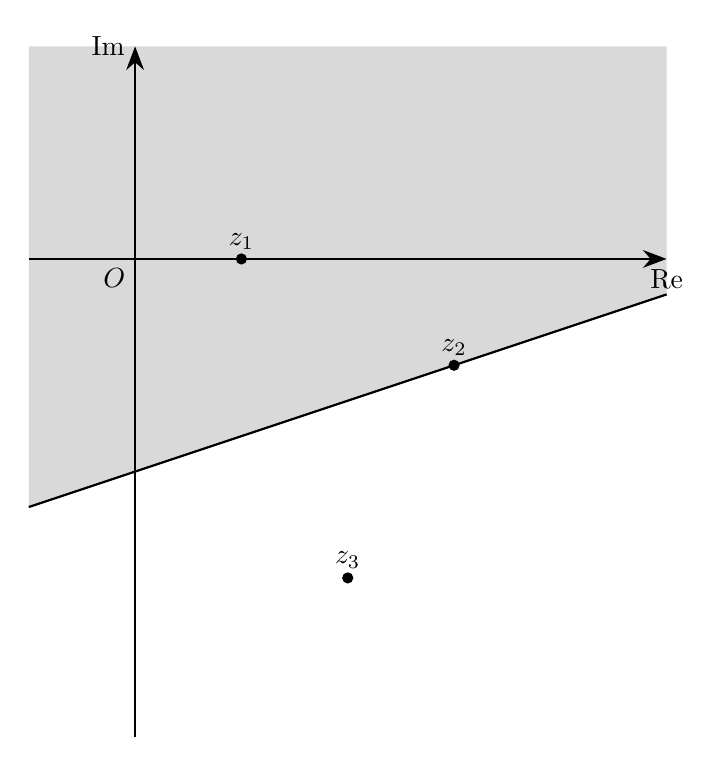
\begin{tikzpicture}[scale=1.35]
\def\xmin{-1}
\def\xmax{5}
\def\ymin{-4.5}
\def\ymax{2}
\def\xone{1}
\def\yone{0}
\def\xtwo{3}
\def\ytwo{-1}
\def\xthree{2}
\def\ythree{-3}
\pgfmathsetmacro{\yleft}{(\xmin-6)/3}
\pgfmathsetmacro{\yright}{(\xmax-6)/3}
\coordinate (O) at (0,0);
\coordinate (z1) at (\xone,\yone);
\coordinate (z2) at (\xtwo,\ytwo);
\coordinate (z3) at (\xthree,\ythree);
\coordinate (L) at (\xmin,\yleft);
\coordinate (R) at (\xmax,\yright);
\begin{scope}
\clip (\xmin,\ymin) rectangle (\xmax,\ymax);
\fill[gray!30] (L) -- (R) -- (\xmax,\ymax) -- (\xmin,\ymax) -- cycle;
\end{scope}
\draw[thick, black, -{Stealth[length=3mm]}] (\xmin,0) -- (\xmax,0) node[below] {$\mathrm{Re}$};
\draw[thick, black, -{Stealth[length=3mm]}] (0,\ymin) -- (0,\ymax) node[left] {$\mathrm{Im}$};
\node[below left] at (O) {$O$};
\draw[thick, black] (L) -- (R);
\foreach \p/\lab in {z1/z_1,z2/z_2,z3/z_3} {
  \fill[black] (\p) circle (1.5pt);
  \node[above] at (\p) {$\lab$};
}
\end{tikzpicture}

The solid boundary is included. Writing \(z=x+iy\), and squaring both non-negative moduli, gives:
\begin{align*}
|z-1|\leqslant |z-2+3i|
&\iff (x-1)^2+y^2\leqslant (x-2)^2+(y+3)^2\\
&\iff x^2-2x+1+y^2\leqslant x^2-4x+4+y^2+6y+9\\
&\iff 2x-6y\leqslant 12\\
&\iff y\geqslant \frac{x-6}{3}
\end{align*}

\end{enumerate}
\end{djsSolution}

\end{enumerate}
\end{document}
